\documentclass[11pt, a4paper, titlepage, openright]{article}

\usepackage{amsmath}
\usepackage[font=small,labelfont=bf]{caption}
\usepackage{float}
\restylefloat{figure}
\usepackage{graphicx}
\usepackage{hyperref}
\usepackage{mathtools}
\usepackage[titletoc, title]{appendix}
\usepackage{listings}
\usepackage{color}
\usepackage{fixltx2e}
\usepackage[bottom]{footmisc}

\usepackage[a4paper, total={6.5in, 9.5in}]{geometry}

\usepackage{eurosym}
\usepackage{graphicx}
\usepackage{wrapfig}
\usepackage{lscape}
\usepackage{rotating}
\usepackage{epstopdf}

\definecolor{dkgreen}{rgb}{0,0.6,0}
\definecolor{gray}{rgb}{0.5,0.5,0.5}
\definecolor{mauve}{rgb}{0.58,0,0.82}

\lstset{frame=tb,
  aboveskip=3mm,
  belowskip=3mm,
  showstringspaces=false,
  columns=flexible,
  basicstyle={\footnotesize\ttfamily},
  numbers=none,
  numberstyle=\tiny\color{gray},
  keywordstyle=\color{blue},
  commentstyle=\color{dkgreen},
  stringstyle=\color{mauve},
  breaklines=true,
  breakatwhitespace=true,
  tabsize=3,
  showstringspaces=false,
  keepspaces=true,
  columns=flexible
  }

\newenvironment{verbquote}
	{\catcode `^=12% Math superscript
	\catcode `_=12% Math subscript
	\catcode `$=12% Math deliniation
	\begin{quote}}
	{\end{quote}}

\begin{document}
%%%%%%%%%%%%%%%%%%%%%%%%%%%%%%%%%%%%%%%%%
% University Assignment Title Page
% LaTeX Template
% Version 1.0 (27/12/12)
%
% This template has been downloaded from:
% http://www.LaTeXTemplates.com
%
% Original author:
% WikiBooks (http://en.wikibooks.org/wiki/LaTeX/Title_Creation)
%
% License:
% CC BY-NC-SA 3.0 (http://creativecommons.org/licenses/by-nc-sa/3.0/)
%
% Instructions for using this template:
% This title page is capable of being compiled as is. This is not useful for
% including it in another document. To do this, you have two options:
%
% 1) Copy/paste everything between \begin{document} and \end{document}
% starting at \begin{titlepage} and paste this into another LaTeX file where you
% want your title page.
% OR
% 2) Remove everything outside the \begin{titlepage} and \end{titlepage} and
% move this file to the same directory as the LaTeX file you wish to add it to.
% Then add \input{./title_page_1.tex} to your LaTeX file where you want your
% title page.
%
%%%%%%%%%%%%%%%%%%%%%%%%%%%%%%%%%%%%%%%%%

%----------------------------------------------------------------------------------------
%	PACKAGES AND OTHER DOCUMENT CONFIGURATIONS
%----------------------------------------------------------------------------------------
\begin{titlepage}

\newcommand{\HRule}{\rule{\linewidth}{0.5mm}} % Defines a new command for the horizontal lines, change thickness here

\center % Center everything on the page

%----------------------------------------------------------------------------------------
%	HEADING SECTIONS
%----------------------------------------------------------------------------------------

\textsc{\LARGE KU Leuven}\\[1.5cm] % Name of your university/college
\textsc{\Large }\\[4cm] % Major heading such as course name
\textsc{\Large Modellering en simulatie}\\[0.5cm] % Minor heading such as course title

%----------------------------------------------------------------------------------------
%	TITLE SECTION
%----------------------------------------------------------------------------------------

\HRule
{ \huge \bfseries Practicum 1:\\ \Large{Monte Carlo-simulaties}}\\ % Title of your document
\HRule \\[1.5cm]

%----------------------------------------------------------------------------------------
%	AUTHOR SECTION
%----------------------------------------------------------------------------------------

\begin{minipage}{0.4\textwidth}
\begin{flushleft} \large
Armin Halilovic - r0679689 % Your name
\end{flushleft}
\end{minipage}
~
\begin{minipage}{0.4\textwidth}
\begin{flushright} \large
\end{flushright}
\end{minipage}\\[4cm]

% If you don't want a supervisor, uncomment the two lines below and remove the section above
%\Large \emph{Author:}\\
%John \textsc{Smith}\\[3cm] % Your name

%----------------------------------------------------------------------------------------
%	DATE SECTION
%----------------------------------------------------------------------------------------

\vfill % Fill the rest of the page with whitespace
{\large 2 December 2016}\\[3cm] % Date, change the \today to a set date if you want to be precise

%----------------------------------------------------------------------------------------
%	LOGO SECTION
%----------------------------------------------------------------------------------------

%\includegraphics{Logo}\\[1cm] % Include a department/university logo - this will require the graphicx package

%----------------------------------------------------------------------------------------


\end{titlepage}
\tableofcontents
\newpage

\section{Oplossingen}
	In deze sectie worden antwoorden op de vragen in het practicum gegeven. De code voor alle opgaven staat onder appendix A.

	\subsection{Geometrische Brownse bewegingen}

	\subsubsection{Opgave 2}
		\begin{quote}
			Bereken de driftfactor \( \mu \) en de volatiliteit \( \sigma \) voor de twee fondsen die je hebt ingeladen in opgave 1 en
			neem deze op in je verslag. Rapporteer 3 beduidende cijfers.
		\end{quote}

		\noindent Output van de code:
\begin{lstlisting}
Driftfactor en volatiliteit voor VTI: 0.00623 en 0.0436
Driftfactor en volatiliteit voor BNP: 0.00466 en 0.0268\end{lstlisting}


	\subsubsection{Opgave 4}
		\begin{quote}
			Simuleer 10 willekeurige paden van het aandelenfonds VTI. Als invoer geef je de \( \mu \) en \( \sigma \)
			die je in opgave 2 berekende, als initialPrice neem je de meest recente marktprijs die je op
			http://www.morningstar.com/stocks/ARCX/VTI/quote.html kunt raadplegen en als lengte van de simulatie
			months kies je 60 maanden. Plot deze tien paden op eenzelfde grafiek. Welke initiele prijs heb je
			gebruikt voor de 10 paden? Vermeld ook de datum. Zien de paden die je gegenereerd hebt er uit
			zoals de koers van VTI van de afgelopen 5 jaar? Motiveer grondig indien je meent van niet.
		\end{quote}

		\noindent De gebruikte initialPrice was \$114.55. Dit was de waarde op 25/11/2016. \\
		Op figuur \ref{fig:vtiPath} is te zien dat de gesimuleerde paden lijken op het werkelijk pad van het aandelenfonds (wel met een ander startpunt).
		De gegenereerde paden zouden nog meer lijken op de koers indien de paden op meer punten zouden worden gesimuleerd (bv per dag ipv per maand).

		\begin{figure}[H]
			\begin{minipage}[b]{0.49\textwidth}
			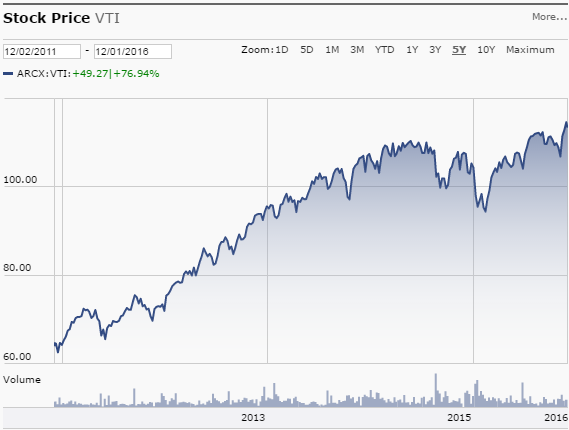
\includegraphics[width=1.0\linewidth]{../ex4-actual}
			\end{minipage}
			\hfill
			\begin{minipage}[b]{0.49\textwidth}
			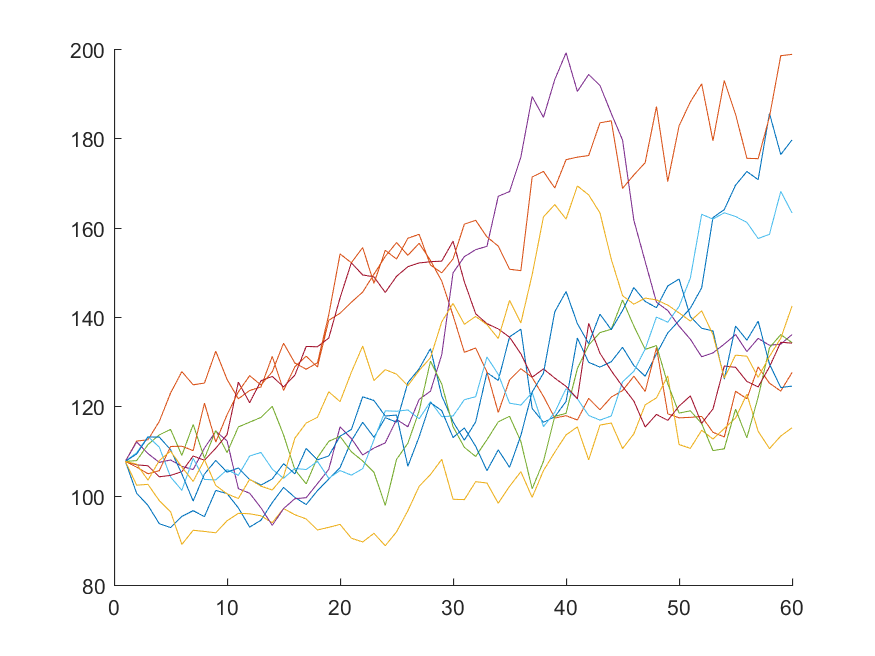
\includegraphics[width=1.0\linewidth]{../ex4-paths}
			\end{minipage}
			\caption{links: werkelijk pad van VTI, rechts: 10 gesimuleerde paden}
			\label{fig:vtiPath}
		\end{figure}

	\newpage
	\subsubsection{Opgave 5}
		\begin{quote}
			Vergelijk de empirische cumulatieve distributiefunctie van de log-rendementen van opeenvolgende maanden
			van het fonds VTI met de cumulatieve distributiefunctie van het model, i.e.,
			\( N(\mu - \frac{1}{2} \sigma^{2}, \sigma^{2}) \). Als modelparameters \( \mu \) en \( \sigma \)
			kies je de overeenkomstige populatiestatistieken die je in opgave 2 hebt berekend. Maak een figuur
			van deze twee functies en neem deze op in het verslag. Kan je op basis van deze figuur besluiten
			dat de geobserveerde log-rendementen van VTI gedurende de laatste 184 maanden inderdaad bij
			benadering voldoen een normale verdeling met gemiddelde \( \mu - \frac{1}{2} \sigma^{2} \) en standaardafwijking \( \sigma^{2} \)?
		\end{quote}

		\noindent Op figuur \ref{fig:ex5} zien we dat de grafieken van de cumulatieve distributiefuncties ongeveer samen vallen.
		Hieruit kunnen we besluiten dat de log-rendementen inderdaad bij benadering voldoen aan
		een normale verdeling met gemiddelde \( \mu - \frac{1}{2} \sigma^{2} \) en standaardafwijking \( \sigma^{2} \).

		\begin{figure}[H]
			\centering
			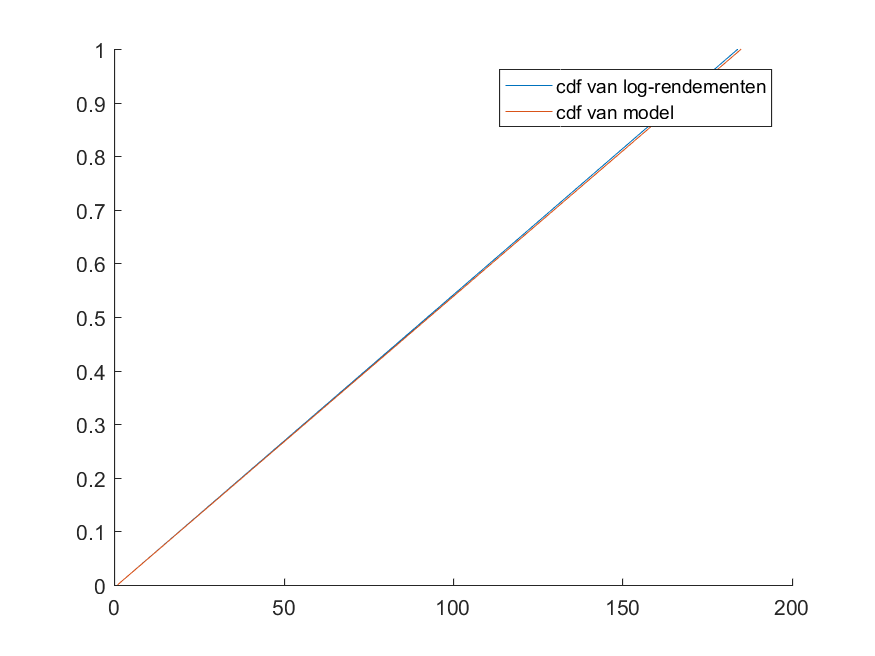
\includegraphics[width=0.7\linewidth]{../ex5}
			\caption{}
			\label{fig:ex5}
		\end{figure}



	\subsection{Simuleren van scenario's voor pensioensparen}

	\subsubsection{Opgave 6}
		\begin{quote}
			Hoeveel geld heb je na 40 kwartalen gestort als je start met een spaarbudget per kwartaal van \euro 500?
		\end{quote}

		\noindent Output van de code:
\begin{lstlisting}
Gestort geld na 40 kwartalen met startbudget van 500 euro: 21899.44\end{lstlisting}

	\newpage
	\subsubsection{Opgave 13}
		\begin{quote}
			 Simuleer het rendement voor elk van de 3 scenario's na 40 kwartalen (10 jaar) wanneer je spaarbudget \euro750
			 per kwartaal bedraagt. Voor de spaarrekening zullen we de extreem gunstige getrouwheidspremie van 3.0\%
			 hanteren. Maak histogrammen van de gesimuleerde rendementen van de fondsen.
			 Hoeveel bedraagt het rendement (uitgedrukt in \%) van de spaarrekening?
		\end{quote}

		\noindent Output van de code:
\begin{lstlisting}
Spaarrekening rendement: 0.118304
Aandelenfonds VTI rendementen: min -0.514990, max 4.734315, mean 0.525865, median 0.452880
Pensioenfonds BNP rendementen: min -0.297107, max 2.142379, mean 0.387006, median 0.363345\end{lstlisting}
		Het rendement van de spaarrekening bedraagt 11.83\% na 10 jaar.

		\begin{figure}[H]
		\centering
		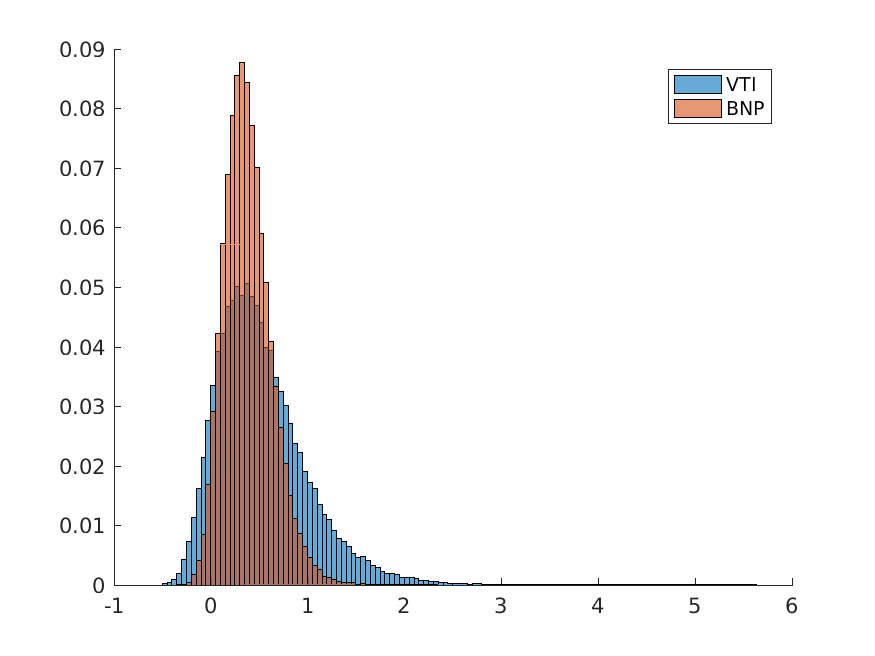
\includegraphics[width=1\linewidth]{../ex13}
		\caption{Histogrammen van rendementen voor de fondsen na 40 kwartalen}
		\label{fig:ex13}
		\end{figure}

	\newpage
	\subsubsection{Opgave 14}
		\begin{quote}
			Voer de voorgaande simulatie ook uit voor \( 4 * (60 - x) \) kwartalen, waarbij x je leeftijd is.
			Maak dezelfde figuur opnieuw en neem deze op in het verslag. Bespreek je resultaten. Valt er iets bijzonder op in deze figuur?
		\end{quote}

		\noindent Output van de code:
\begin{lstlisting}
Spaarrekening rendement: 0.559096
Aandelenfonds VTI rendementen: min -0.587350, max 126.814567, mean 5.310819, median 3.916414
Pensioenfonds BNP rendementen: min -0.334121, max 18.799478, mean 2.205920, median 1.954154\end{lstlisting}
		De gebruikte \( x \) was 22. \\
		Het rendement van de spaarrekening bedraagt 55.91\% na 38 jaar. Het verschil tussen het rendement van de spaarrekening en de
		gemiddelde rendementen van de fondsen is sterk gestegen. Daarnaast is het ook opmerkbaar dat er heel erg grote rendementen mogelijk
		zijn met het VTI aandelenfonds, terwijl het mogelijk verlies maar amper is toegenomen.


		\begin{figure}[H]
			\centering
			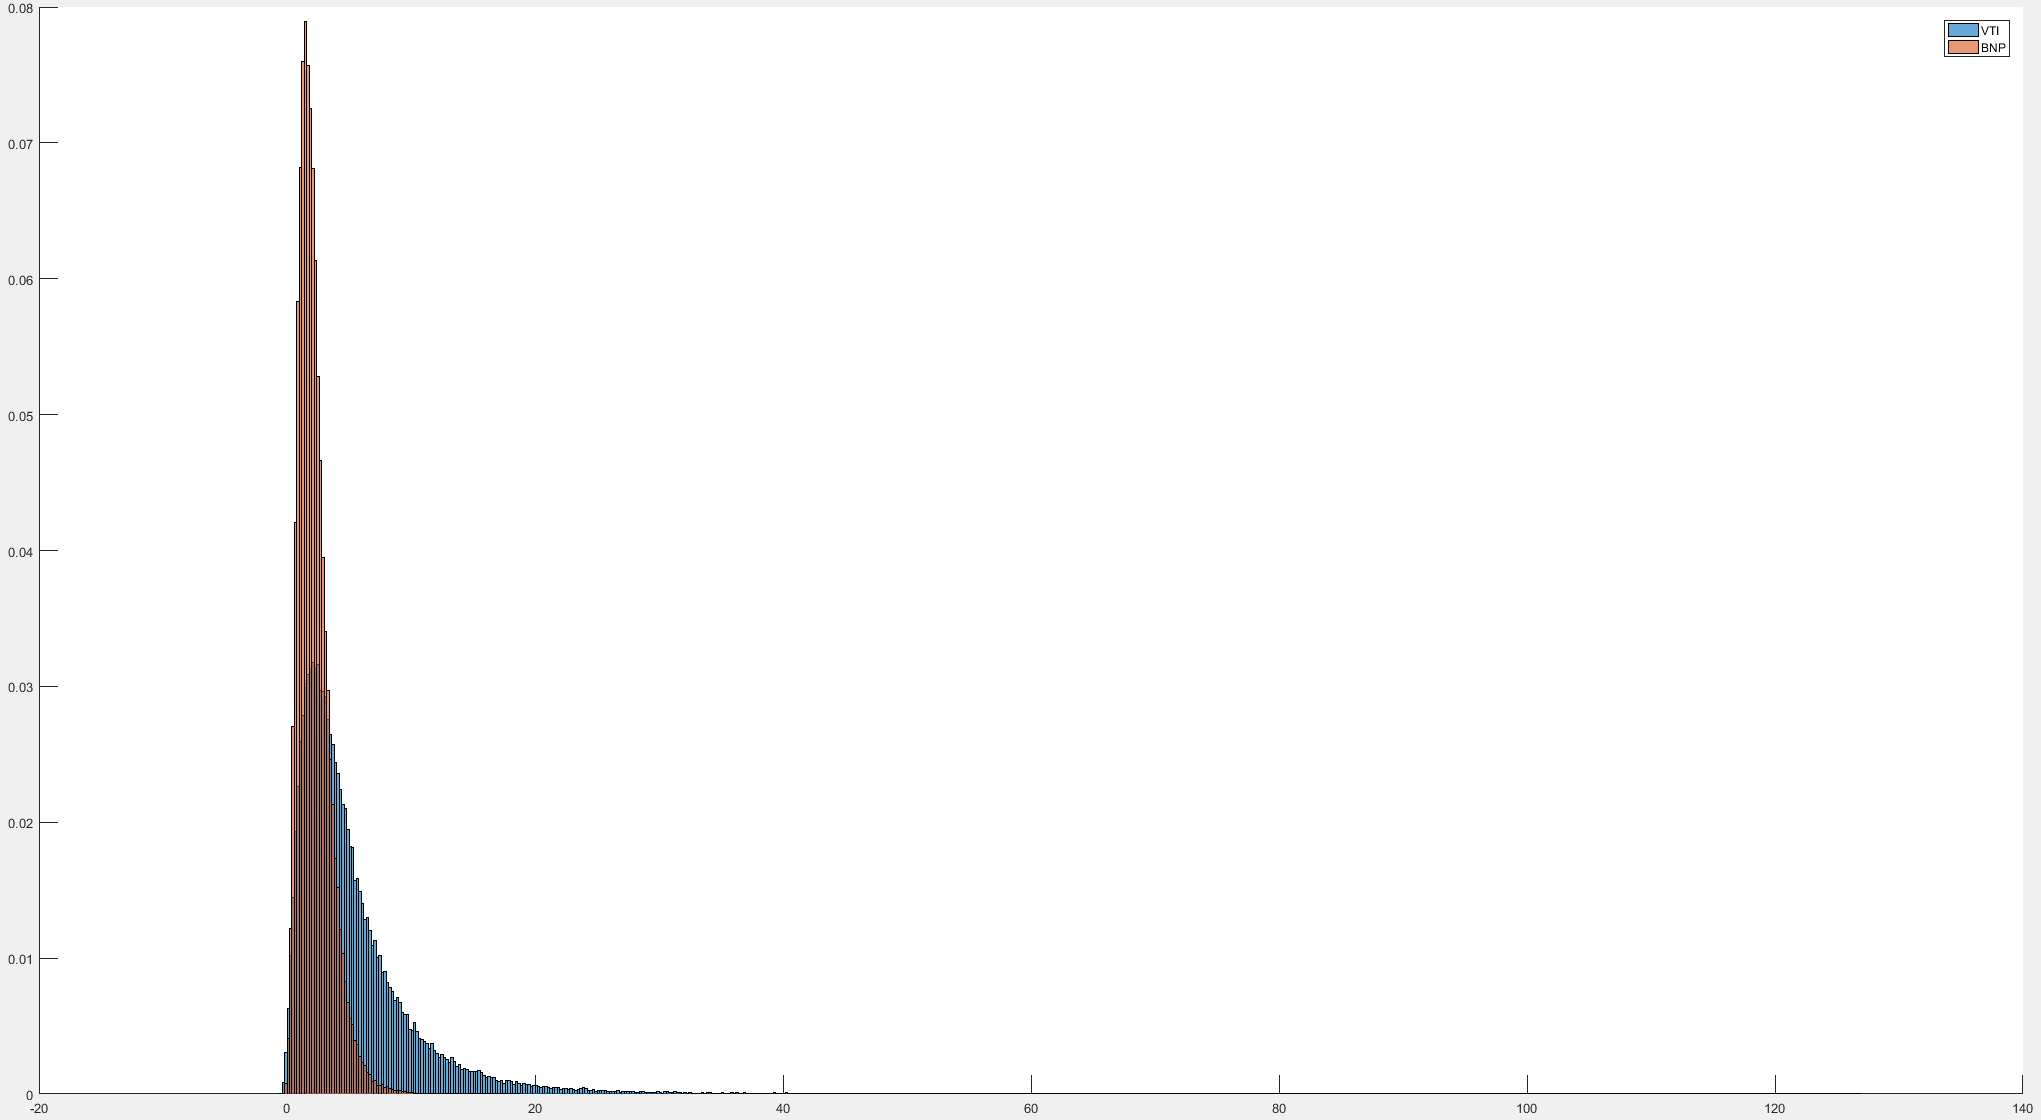
\includegraphics[width=1\linewidth]{../ex14-backup}
			\caption{Histogrammen van rendementen voor de fondsen na 152 kwartalen}
			\label{fig:ex14}
		\end{figure}

	\iffalse
	\subsubsection{Opgave 15}
		\begin{quote}
			Simuleer het rendement voor elk van de 3 scenario's na 40, 80, 120 en 160 kwartalen wanneer je spaarbudget steeds \( (250+x) \)
			euro per kwartaal bedraagt, waarbij x de laatste 3 cijfers van je studentennummer zijn. Rapporteer x in het verslag.
			Hoe groot is de kans om een negatief eindrendement te behalen in de 3 scenario's en voor de 4 verschillende lengtes van de simulatie?
			Geef je antwoord in een duidelijke tabel. Hoeveel bedraagt de kans om een vermogen van minstens \euro1 miljoen opgebouwd te hebben in elk van deze 12 simulaties? Maak opnieuw een tabel.
		\end{quote}
	\fi

	\newpage
	\subsubsection{Opgave 16}
		\begin{quote}
			Simuleer het rendement van het BNP-pensioenfonds na 160 kwartalen wanneer je de volgende spaarbudgetten (per kwartaal)
			zou aanhouden: \euro125, \euro250, \euro500, \euro1000 en \euro2000. Hoeveel bedraagt de mediaan van het eindrendement
			in deze vijf gevallen? Wat valt op? Verklaar dit bijzondere fenomeen.
		\end{quote}

		\noindent Output van de code:
\begin{lstlisting}
Gegevens over de eindrendementen: min 2.236039, max 3.299977, mean 2.681874, median 2.557744\end{lstlisting}
		De mediaan van het eindrendement in de vijf gevallen bedraagt 2.56. Ik merk echter geen bijzonder fenomeen op.

		\begin{figure}[H]
		\begin{minipage}[b]{0.49\textwidth}
		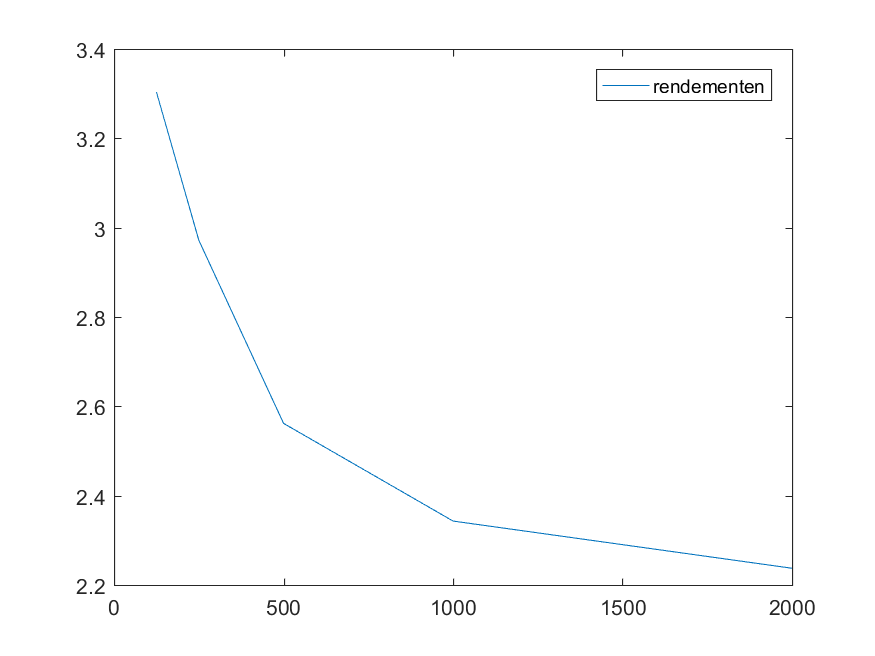
\includegraphics[width=1.0\linewidth]{../ex16}
		\end{minipage}
		\hfill
		\begin{minipage}[b]{0.49\textwidth}
		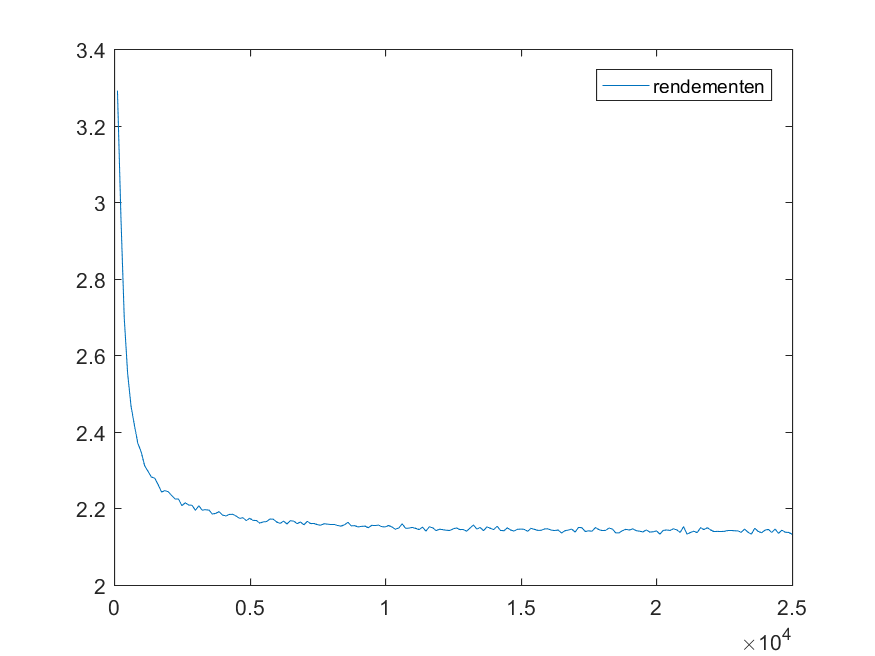
\includegraphics[width=1\linewidth]{../ex16-veel-budgetten}
		\end{minipage}
		\caption{links: rendementen met de gegeven budgetten, rechts: rendementen met budgetten tot 25000}
		\label{fig:ex16}
		\end{figure}

	\subsubsection{Opgave 17}
		\begin{quote}
			Bij welk spaarbudget per kwartaal haal je het hoogste verwachte eindrendement wanneer je
			in het wettelijk stelsel van pensioensparen je geld belegt in het 'BNP Paribas B Pension Balanced Classic' fonds?
		\end{quote}

		\noindent Het hoogste verwachtte rendement wordt behaald wanneer de teruggave via de belastingsaangifte en
		de waarde van het fonds (op het laatste moment) maximaal zijn. Hiervan kunnen we enkel het eerste besturen. \\
		De eerste teruggave (\( = taxReturnRate * sum(investments(q-5:q-2)) \)) moet dus gelijk zijn aan \euro282.
		Dit gebeurt wanneer het budget gelijk is aan \euro 235. In dat geval investeer je in je eerste jaar \euro 940 en
		krijg je het daaropvolgende jaar een maximale teruggave.

	\newpage
	\subsubsection{Opgave 18}
		\begin{quote}
			Simuleer het rendement van het VTI-fonds na 160 kwartalen wanneer je de volgende spaarbudgetten
			(per kwartaal) zou aanhouden: \euro125, \euro250, \euro500, \euro1000 en \euro2000. Hoeveel bedraagt de
			mediaan van het eindrendement in deze vijf gevallen? Wat valt op? Verklaar.
		\end{quote}


		\noindent Output van de code:
\begin{lstlisting}
Gegevens over de eindrendementen: min 5.684835, max 6.129065, mean 5.959699, median 5.987950\end{lstlisting}
		De mediaan van het eindrendement in de vijf gevallen bedraagt 5.96.

		\begin{figure}[H]
		\begin{minipage}[b]{0.49\textwidth}
		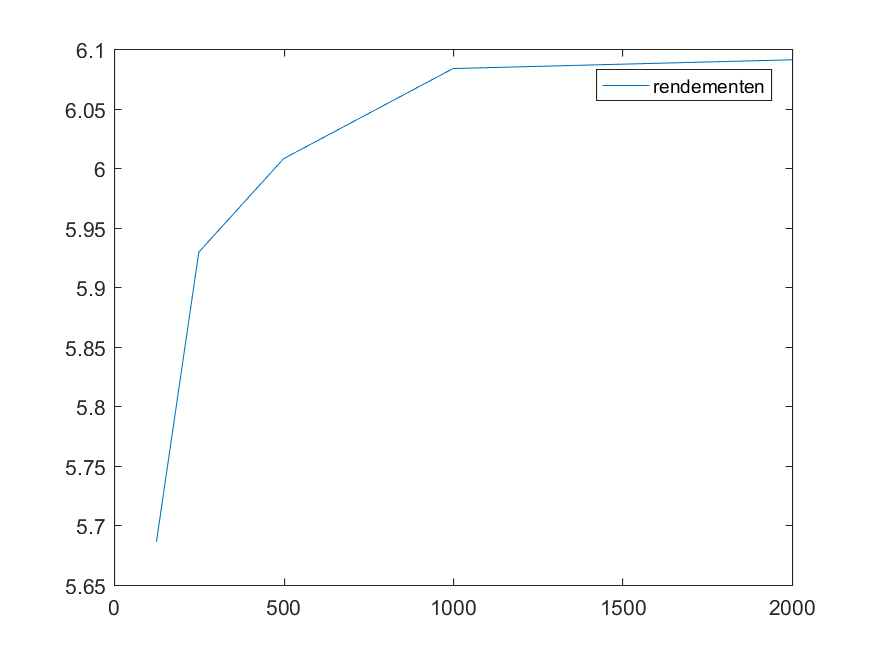
\includegraphics[width=1.0\linewidth]{../ex18}
		\end{minipage}
		\hfill
		\begin{minipage}[b]{0.49\textwidth}
		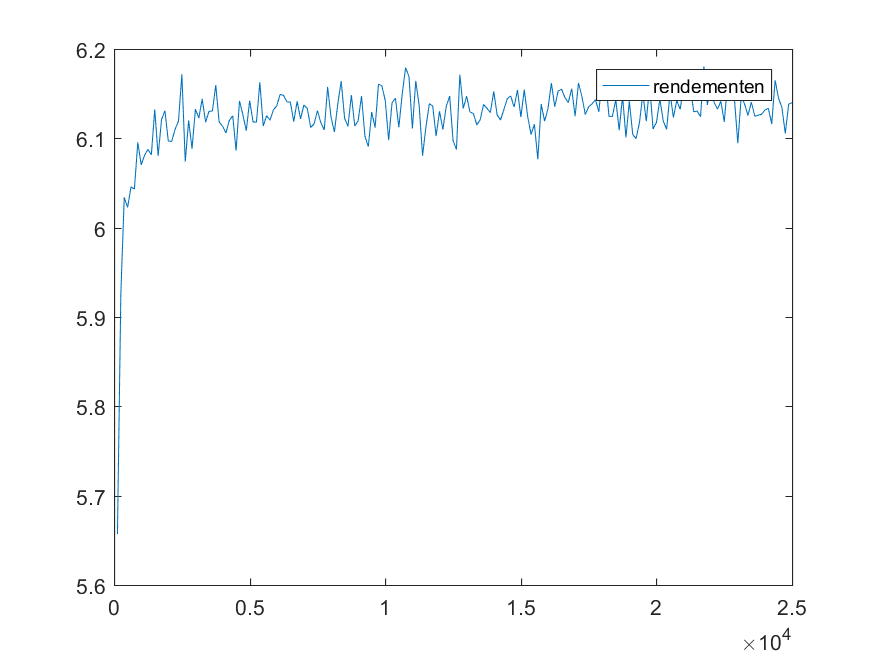
\includegraphics[width=1\linewidth]{../ex18-veel-budgetten}
		\end{minipage}
		\caption{links: rendementen met de gegeven budgetten, rechts: rendementen met budgetten tot 25000}
		\label{fig:ex18}
		\end{figure}

	\subsubsection{Opgave 19}
		\begin{quote}
			Bij welk spaarbudget per kwartaal haal je het hoogste verwachte eindrendement wanneer je je geld belegt in het
			'Vanguard Total Stock Market Index Fund' fonds?
		\end{quote}

		\noindent Vanuit de linkse grafiek in figuur \ref{fig:ex18} lijkt het mogelijk om een ongelimiteerd eindrendement te behalen. Op de rechtergrafiek valt echter
		op dat er een limiet lijkt te zijn op het eindrendement met een waarde rond 6.13. Dit is ongeveer een bedrag van \euro3500.

		\iffalse
		Dit kan worden verklaard met behulp van figuur \ref{fig:vtiPath2}. Op een gegeven moment begint de total nettoinventariswaarde van het fonds sterk te stijgen en
		blijft het die stijging aanhouden tot het einde van de simulatie. Dit betekent wel dat het aankopen van nieuwe aandelen (\( budgetNet / pricePath(q) \)) minder aandelen oplevert (omdat pricePath(q) snel groeit).

		\begin{figure}[H]
			\centering
			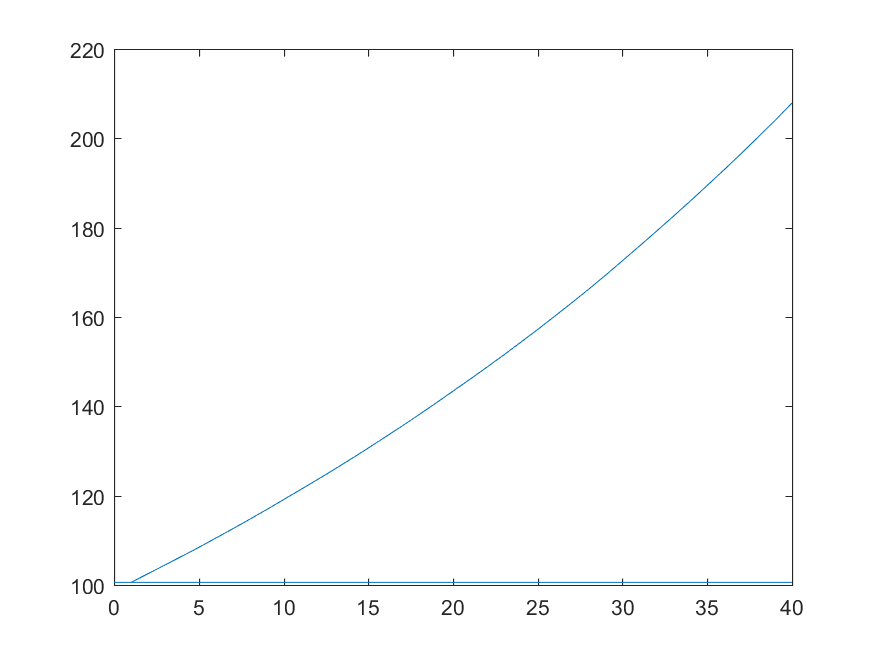
\includegraphics[width=0.5\linewidth]{../vtiPath-100000}
			\caption{Het gemiddelde pad van het VTI fonds met 100 000 simulaties}
			\label{fig:vtiPath2}
		\end{figure}
		\fi


	\subsubsection{Opgave 20}
		\begin{quote}
			Alle voorgaande experimenten indachtig, welke strategie zou jij aanbevelen voor pensioensparen?
			Dit mag een combinatie van meerdere technieken zijn.
		\end{quote}

		\noindent Uitgaande van de simulaties in opgave 14 en figuur \ref{fig:ex14} zou ik aanbevelen om in een aantal distributiefondsen gelijkaardig aan VTI te investeren.
		Op de grafiek is zichtbaar dat in deze simulatie er gigantisch veel winst mogelijk is terwijl het maximaal mogelijk verlies relatief weinig is.
		Als er verlies wordt geleden met een fonds, dan zal hoogstwaarschijnlijk de winst met een ander fonds dat verlies tegengaan.



	\subsection{Evaluatie}

	\subsubsection{Opgave 21}
		\begin{quote}
			Hoeveel tijd heb je gespendeerd aan het oplossen van de opdrachten?
			Hoeveel tijd heb je gespendeerd aan het schrijven van het verslag?
		\end{quote}
		\noindent Ik heb ongeveer 19 uur gespendeerd aan het oplossen van de opdracht en 4 uur aan het schrijven van het verslag.

	\subsubsection{Opgave 22}
		\begin{quote}
			Denk je dat de resultaten van dit practicum realistisch zijn? Hebben de resultaten je verrast?
			Zou je zelf een vermogen willen opbouwen via het wettelijke stelsel?
			Waarom wel of niet? Welke strategie zou je zelf verkiezen?
		\end{quote}
		\noindent Ik heb het gevoel dat de resultaten niet realistisch zijn, waarschijnlijk door dat ik ergens fouten heb gemaakt. Er lijkt een heel grote kans op grote winst te zijn in het VTI fonds, terwijl de kans op verlies vrij klein is. \\
		Zelf weet ik nog niet welke strategie is zou verkiezen, maar het is zeker iets waar ik later meer research moet over doen. Ik heb zeker nuttige dingen bijgelerd om een betere keuze te kunnen maken.


	\subsubsection{Opgave 23}
		\begin{quote}
			Welke bedenkingen heb je bij dit practicum? Was de opgave (veel) te gemakkelijk, (veel) te moeilijk of
			van een gepaste moeilijkheidsgraad? Wat zou je zelf anders aangepakt hebben?  Was de terminologie voldoende duidelijk?
		\end{quote}
		\noindent De moeilijkheidsgraad van dit practicum lijkt me in orde. Ik heb ongeveer even veel tijd gespendeerd als aan het
		eerste practicum (van de 2) van een ander vak van 6 studiepunten.\\
		De terminologie was voldoende duidelijk, maar af en toe waren de specificaties onduidelijk.
		Bijvoorbeeld waar pas je het dividendrendement op toe om de dividend te berekenen? \\ Of moet voor de rendementen
		nog rekening gehouden worden met eindbelastingen? Ergens staat "De eindbelasting nemen we niet op in onze simulatie",
		maar dit lijkt me onlogisch aangezien het geld dat je werkelijk terug zou krijgen lager is dan path(end) en de
		eindbelasting verschillend is voor de verschillende fondsen in de opgave).



\onecolumn
\appendix
\appendixpage
\addappheadtotoc

\section{Code}
	\subsection{Opgaves}
		\subsubsection{Opgave 2}
			\lstinputlisting[basicstyle=\scriptsize]{../r0679689_estimateParameters.m}
			\lstinputlisting[basicstyle=\scriptsize]{../ex2.m}
		\bigskip
		\subsubsection{Opgave 3}
			\lstinputlisting[basicstyle=\scriptsize]{../r0679689_simulatePath.m}
		\bigskip
		\subsubsection{Opgave 4}
			\lstinputlisting[basicstyle=\scriptsize]{../ex4.m}

		\bigskip
		\subsubsection{Opgave 5}
			\lstinputlisting[basicstyle=\scriptsize]{../ex5.m}
		\bigskip
		\subsubsection{Opgave 6}
			\lstinputlisting[basicstyle=\scriptsize]{../r0679689_investedCapital.m}
			\lstinputlisting[basicstyle=\scriptsize]{../ex6.m}
		\bigskip
		\subsubsection{Opgave 7}
			\lstinputlisting[basicstyle=\scriptsize]{../r0679689_simulateSaving.m}
		\bigskip
		\subsubsection{Opgave 8}
			\lstinputlisting[basicstyle=\scriptsize]{../r0679689_simulateQuarterlyPath.m}
		\bigskip
		\subsubsection{Opgave 9}
			\lstinputlisting[basicstyle=\scriptsize]{../r0679689_simulateFundInvestingPath.m}
		\bigskip
		\subsubsection{Opgave 10}
			\lstinputlisting[basicstyle=\scriptsize]{../r0679689_simulateFundInvesting.m}
		\bigskip
		\subsubsection{Opgave 11}
			\lstinputlisting[basicstyle=\scriptsize]{../r0679689_simulatePensionFundInvestingPath.m}
		\bigskip
		\subsubsection{Opgave 12}
			\lstinputlisting[basicstyle=\scriptsize]{../r0679689_simulatePensionFundInvesting.m}
		\bigskip
		\subsubsection{Opgave 13}
			\lstinputlisting[basicstyle=\scriptsize]{../ex13.m}
		\bigskip
		\subsubsection{Opgave 14}
			\lstinputlisting[basicstyle=\scriptsize]{../ex14.m}
		\bigskip
		\subsubsection{Opgave 15}
			\lstinputlisting[basicstyle=\scriptsize]{../ex15.m}
		\bigskip
		\subsubsection{Opgave 16}
			\lstinputlisting[basicstyle=\scriptsize]{../ex16.m}
		\bigskip
		\subsubsection{Opgave 18}
			\lstinputlisting[basicstyle=\scriptsize]{../ex18.m}
		\bigskip

	\subsection{Extra Functies}
		\subsubsection{r0679689\_brownianMove}
			\lstinputlisting[basicstyle=\scriptsize]{../r0679689_brownianMove.m}
		\bigskip
		\subsubsection{r0679689\_compareSavingsAlternatives}
			\lstinputlisting[basicstyle=\scriptsize]{../r0679689_compareSavingsAlternatives.m}
		\bigskip
		\subsubsection{r0679689\_logYields}
			\lstinputlisting[basicstyle=\scriptsize]{../r0679689_logYields.m}
		\bigskip

\end{document}



\iffalse
	We are given the function
	\[
		\begin{aligned}
		f(x) = 1 + T_6(x)    && -1 \le x \le 1
		\end{aligned}
	\]

	where \(T_6(x)\) is the Chebyshev polynomial of degree 6.
	We are tasked to calculate the exact integral \[ I = \int_{-1}^1 \! f(x) \, \mathrm{d}x \] using Maple.
	Also, we are tasked to calculate following numerical approximations using Matlab for up to 2 significant numbers:
	\begin{itemize}
		\item The composite trapezoid rule for \( I \)
		\item \( I \) via a Gauss-Legendre integration rule
		\item Monte Carlo integration of  \( I \)
	\end{itemize}

	\begin{figure}[H]
		\begin{minipage}[b]{0.49\textwidth}
			% \includegraphics[width=1.0\textwidth]{../maple/mapleChebyPlot.png}
		\end{minipage}
		\hfill
		\begin{minipage}[b]{0.49\textwidth}
			\end{minipage}
		\caption{Two plots of the given function.}
		\label{fig:function}
	\end{figure}

	\begin{lstlisting}
		f := x -> 1 + ChebyshevT(6, x);
		int(f(x), x = -1 .. 1);
	\end{lstlisting}
\fi
